% header
\documentclass[10pt,a4paper]{article}

\usepackage[utf8]{inputenc}
\usepackage{hyperref}
\usepackage{amssymb}
\usepackage{amsmath}
\usepackage{listings}
\usepackage{graphicx}

% the document
\begin{document}

\title{Worksheet $4$\\
\small{Practical Lab Numerical Computing}}
\author{Andrii Lischishin \and Lars Schleithoff \and Hendrik Kleikamp}
\date{\today}
\maketitle

\section*{Task 1}

\begin{center}
	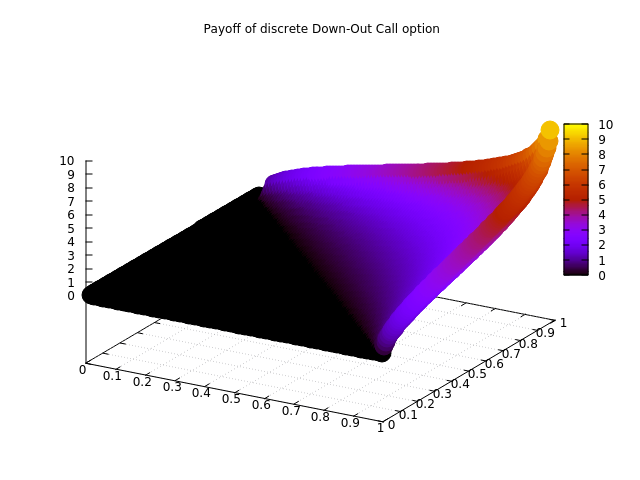
\includegraphics[scale=0.7]{payoff_down_out_call.png}
\end{center}

\section*{Task 2}


\begin{center}
	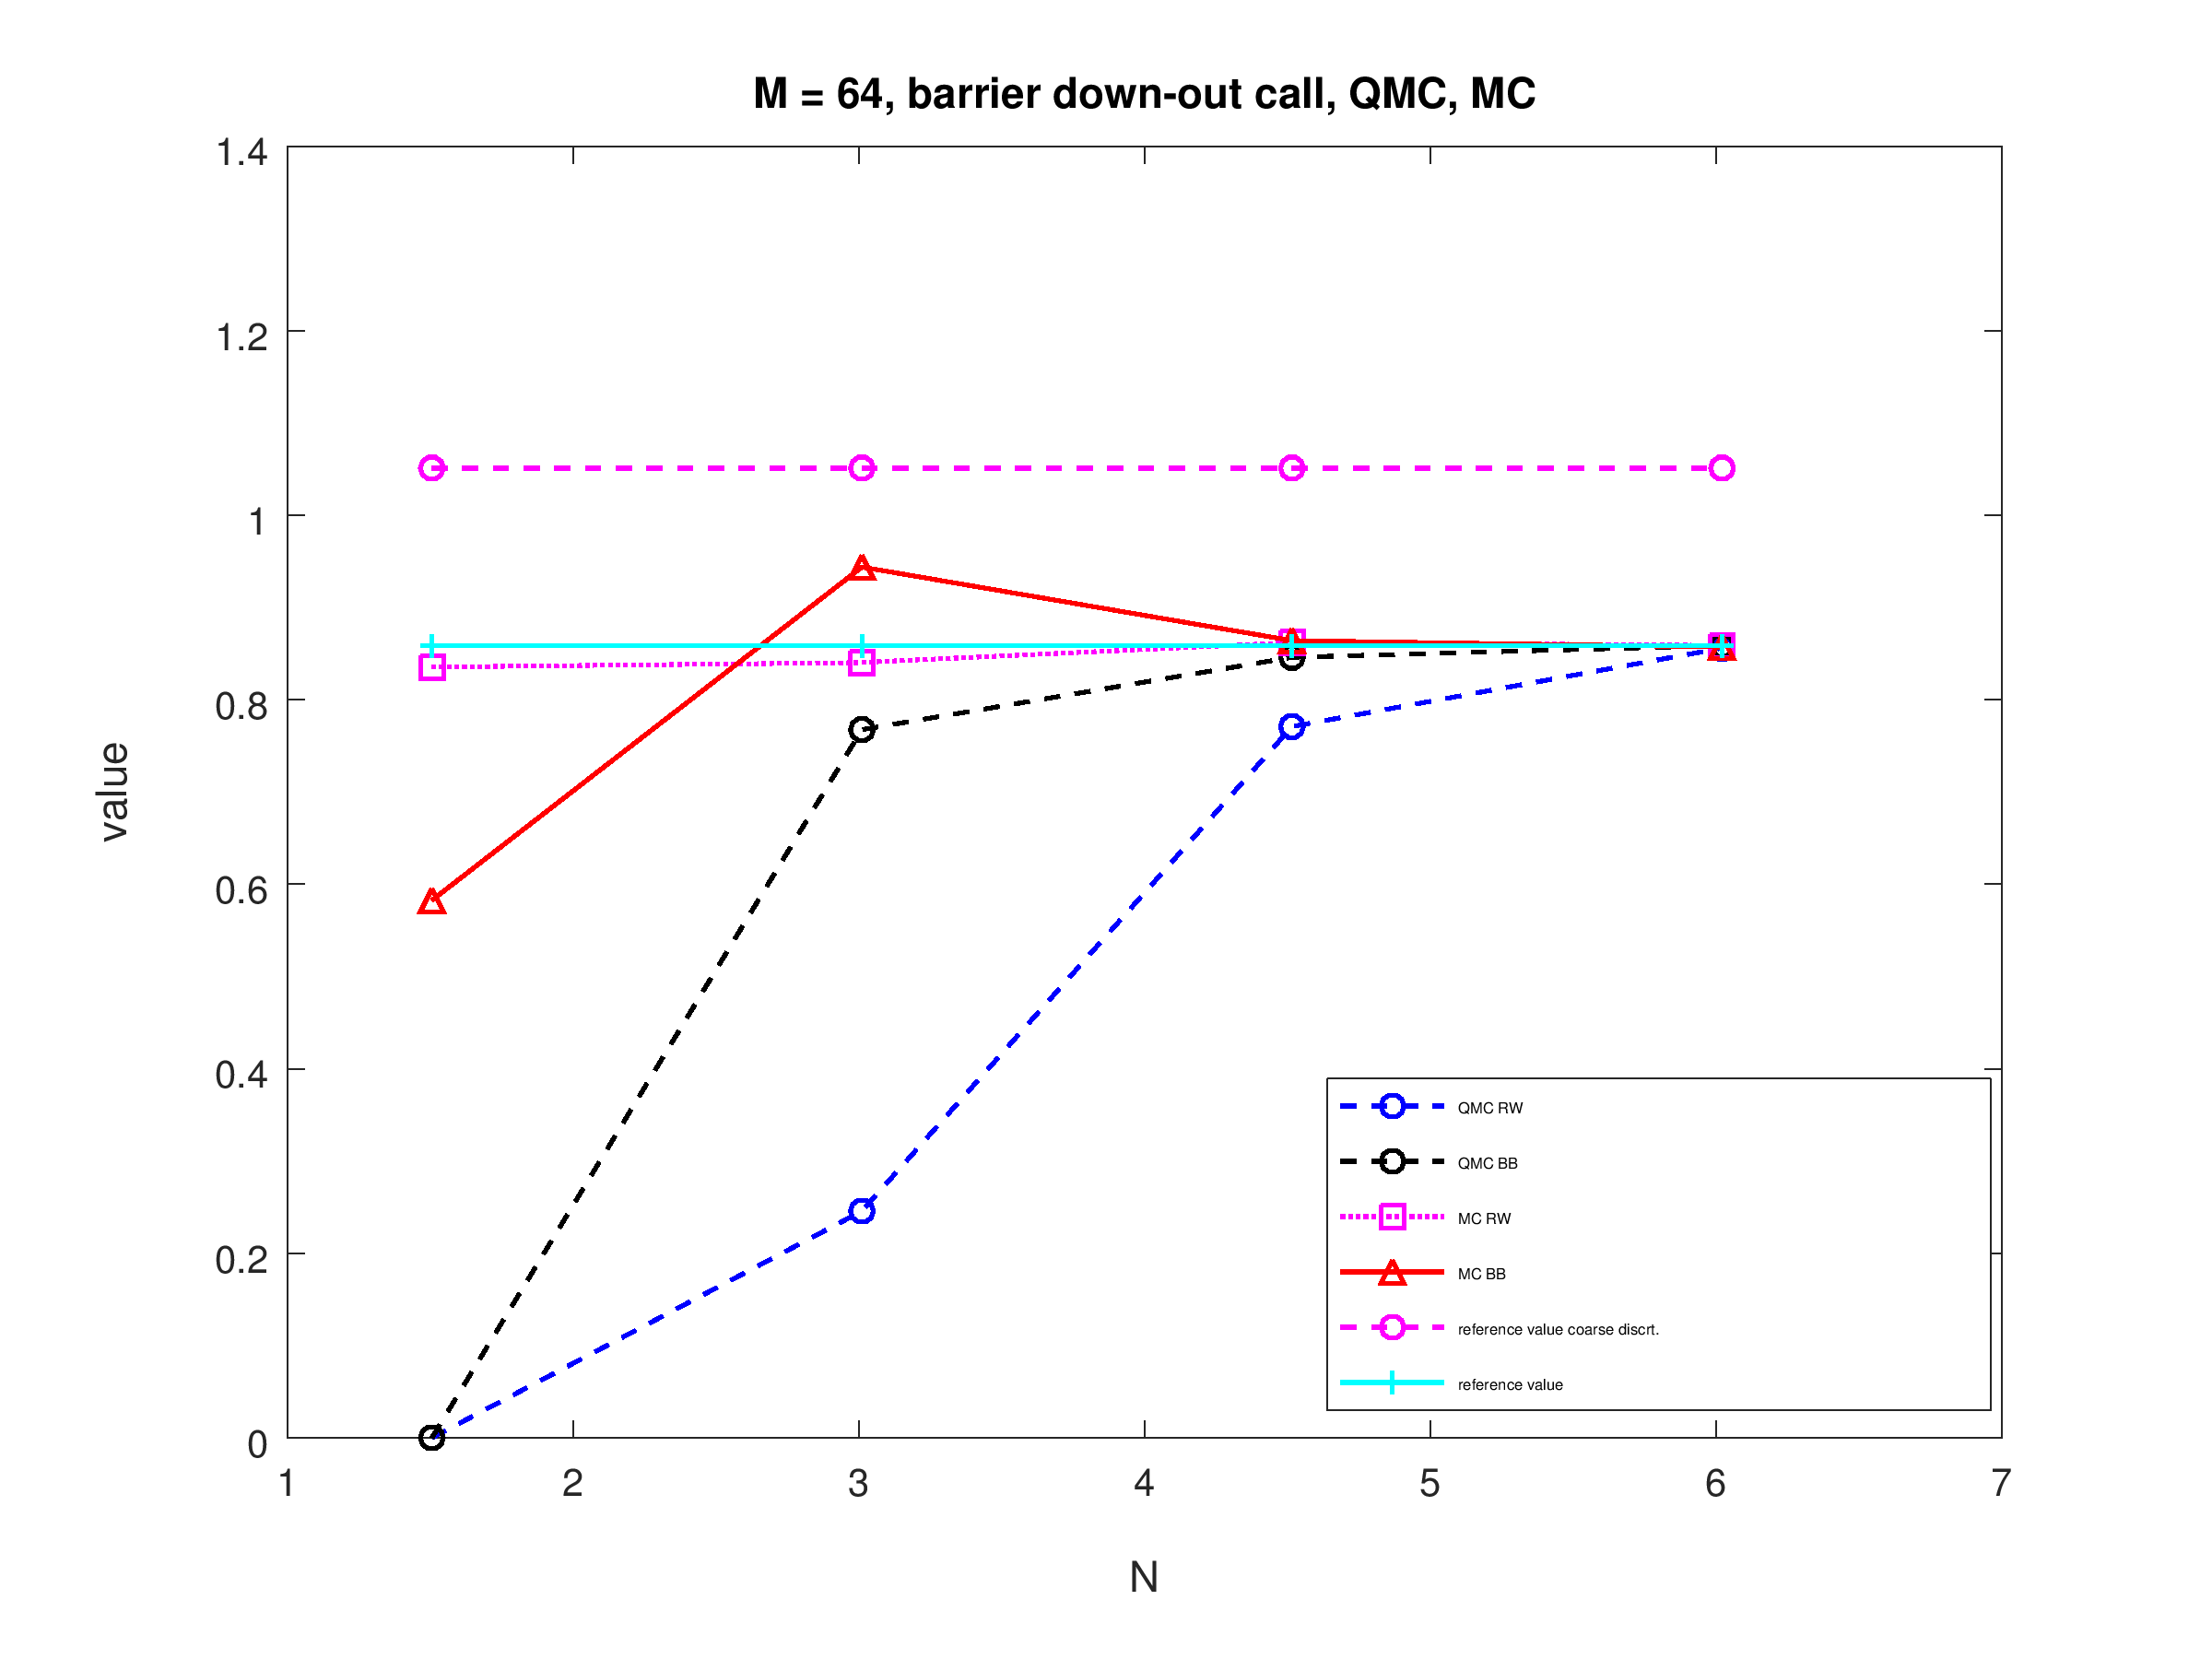
\includegraphics[scale=0.3]{images/task2.png}
\end{center}

\begin{itemize}
    \item{On this figure the value of Barrier Down-Out Call Option using different methods is plotted against number of points($10^N$)
    }
\item{
The pink dashed line is the reference value obtained if precision is too low. So, if precision is too low, the reference value lies above or below the actual price.
}
\item{
From the plots, one can observe that for QMC Brownian-Bridge shows faster convergence than Random-Walk, but for MC it is vice versa
}
\end{itemize}
\newpage
The next figure represents error convergence rates of the above figure:

\begin{center}
	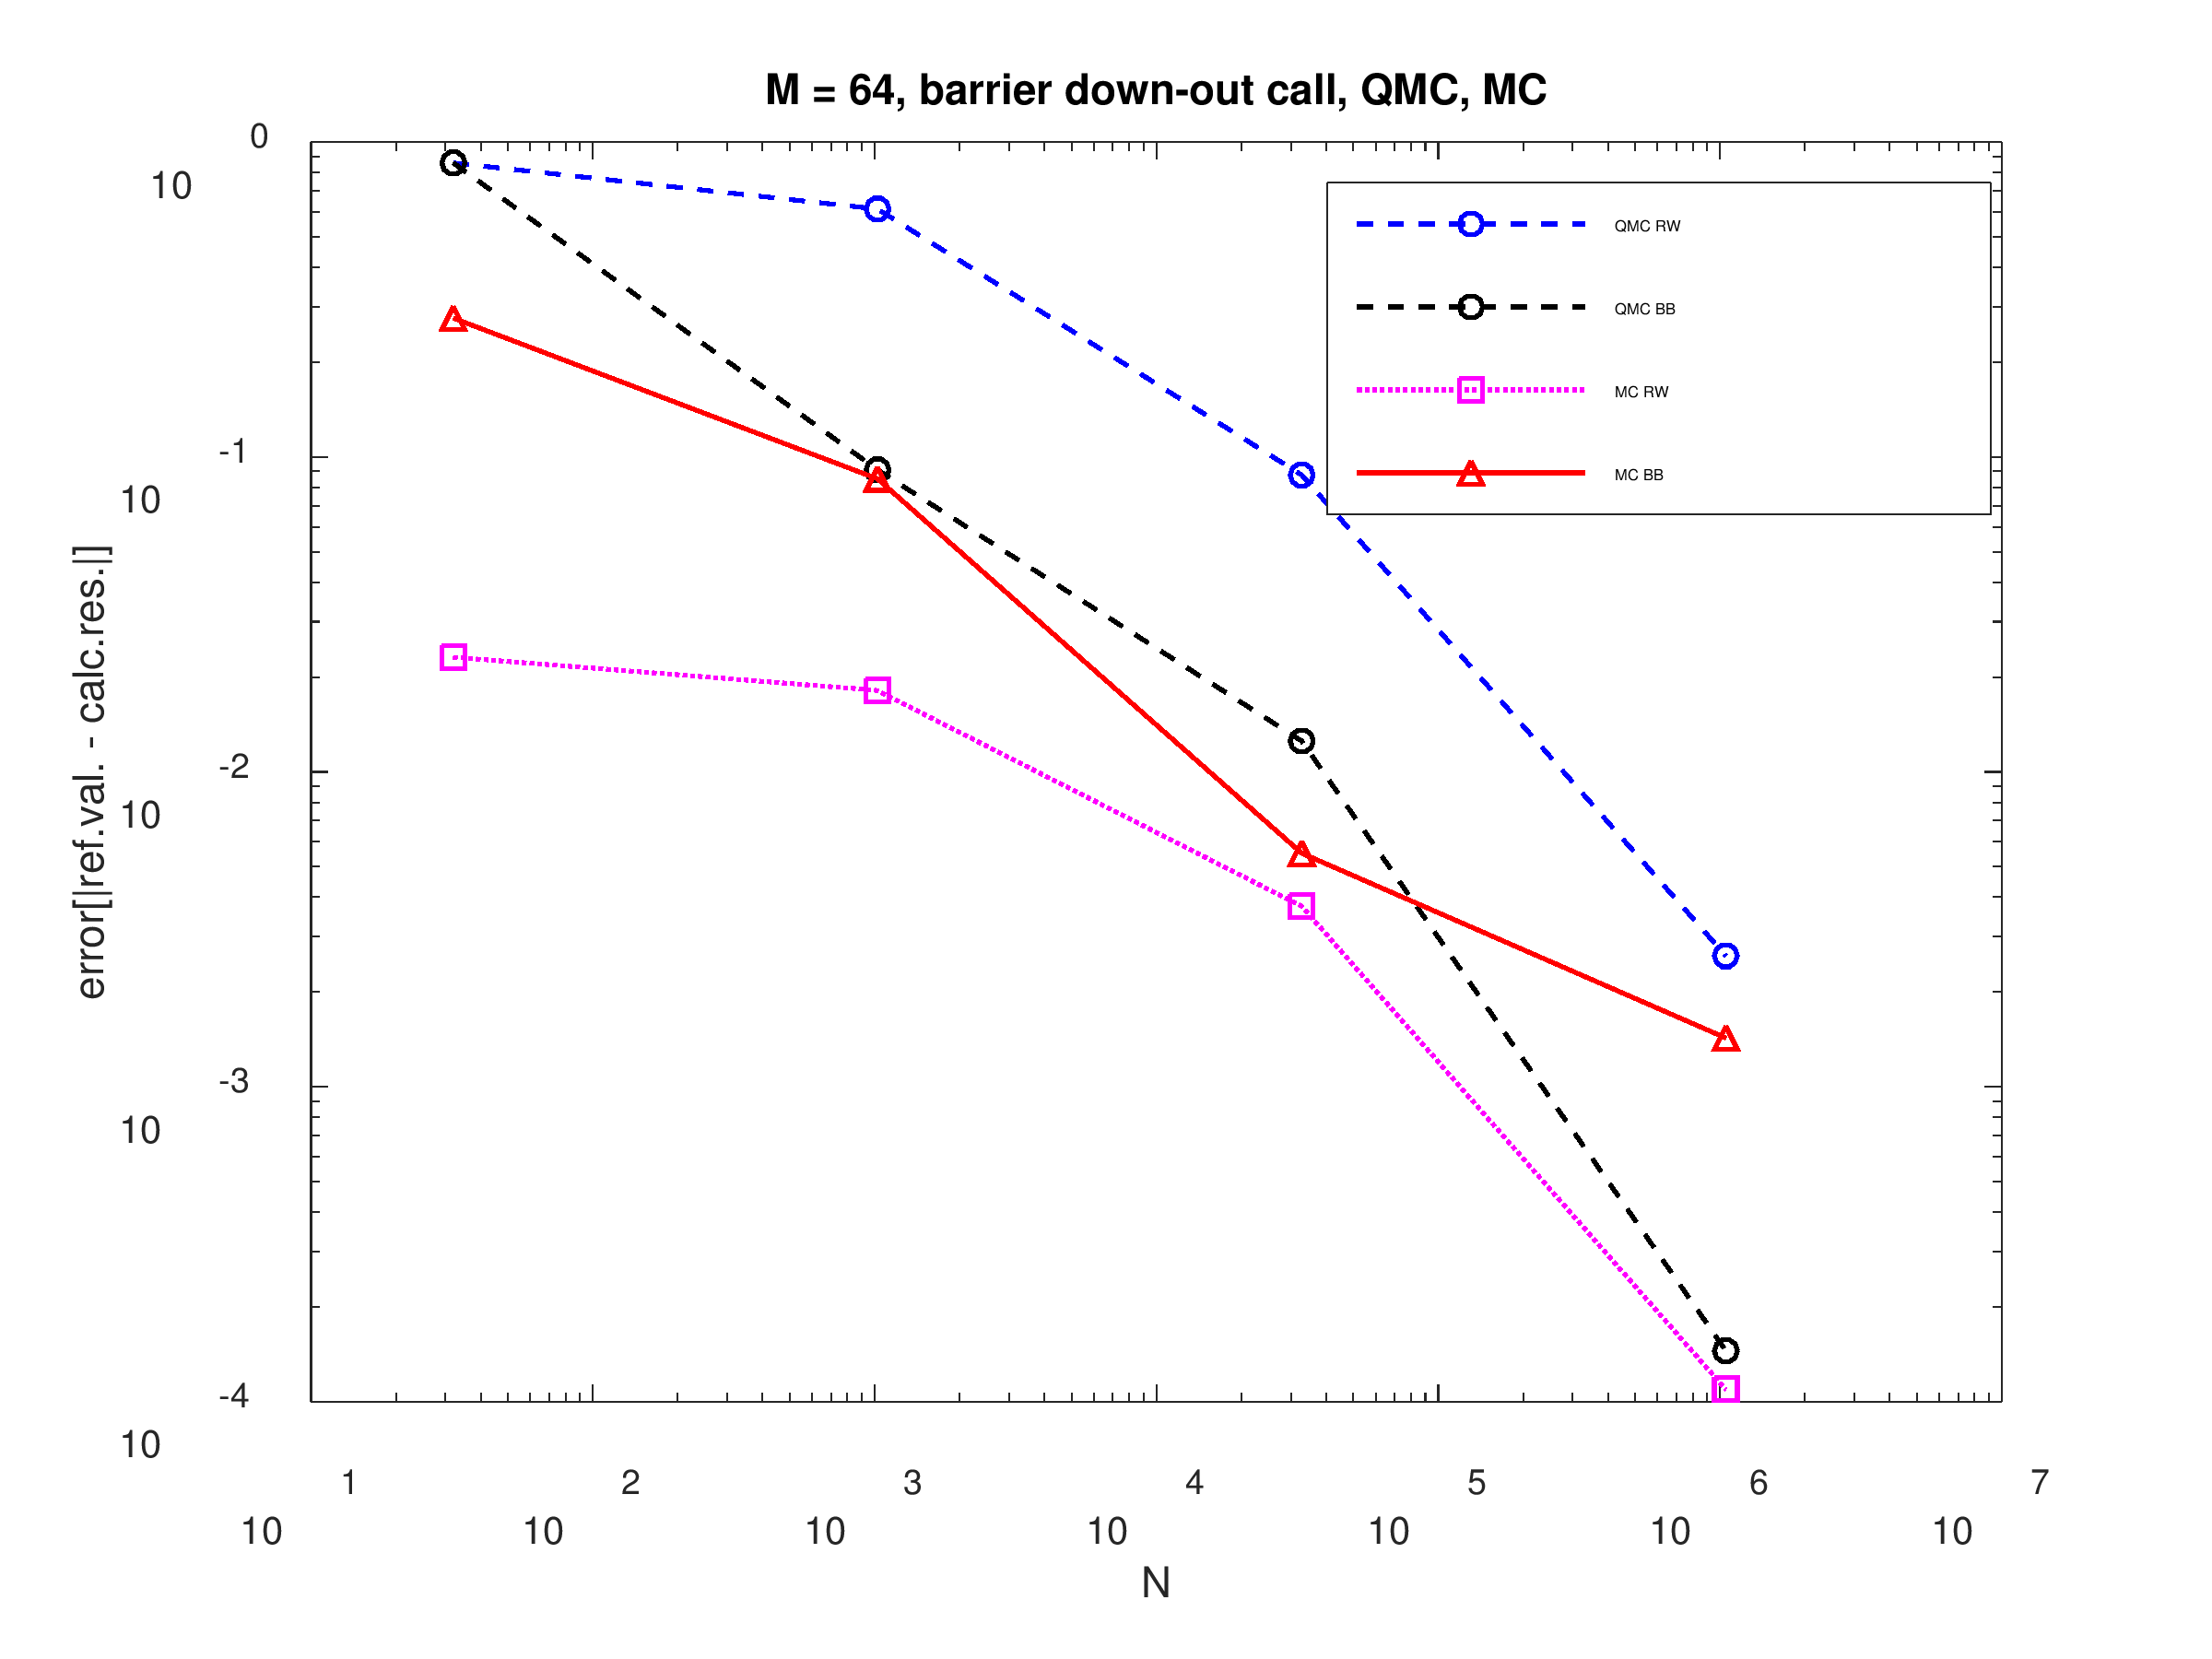
\includegraphics[scale=0.35]{images/task2_error.png}
\end{center}

\section*{Task 3}

The picture below shows the fair price for a Down-Out call option with barrier $B$. One can see that the fair price is going down if the barrier is larger then about $B=8$. This makes sense, because when the barrier is high, the payoff is $0$ in many cases (because for this value of $B$ it happens more often that the price of the underlying is below the barrier).

\begin{center}
	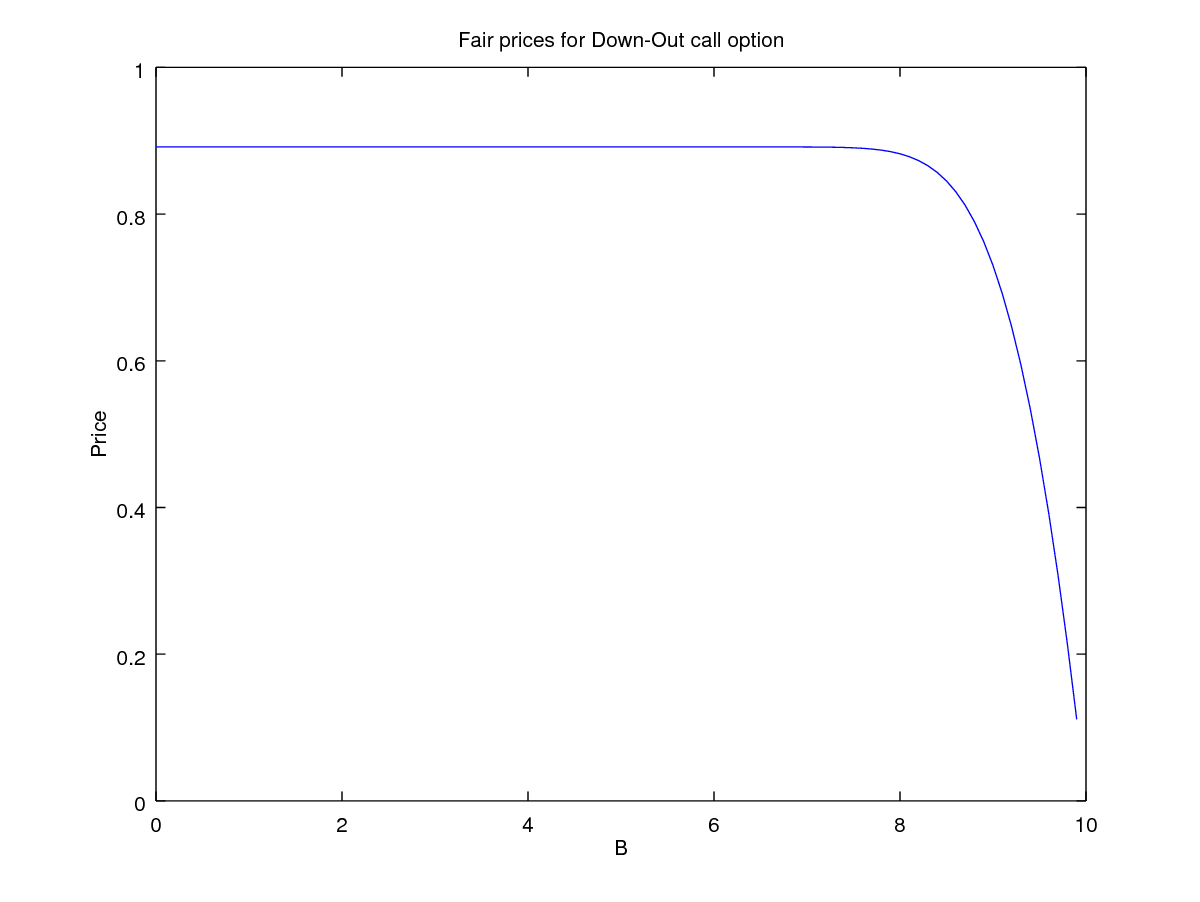
\includegraphics[scale=0.4]{fair_prices_down_out_call.png}
\end{center}

\section*{Task 4}

The next plot shows the absolute error for the discrete Down-Out call option for different values of $M$. One can see that for $M\geq64$ the convergence is much better then for $M=4$.  

\begin{center}
	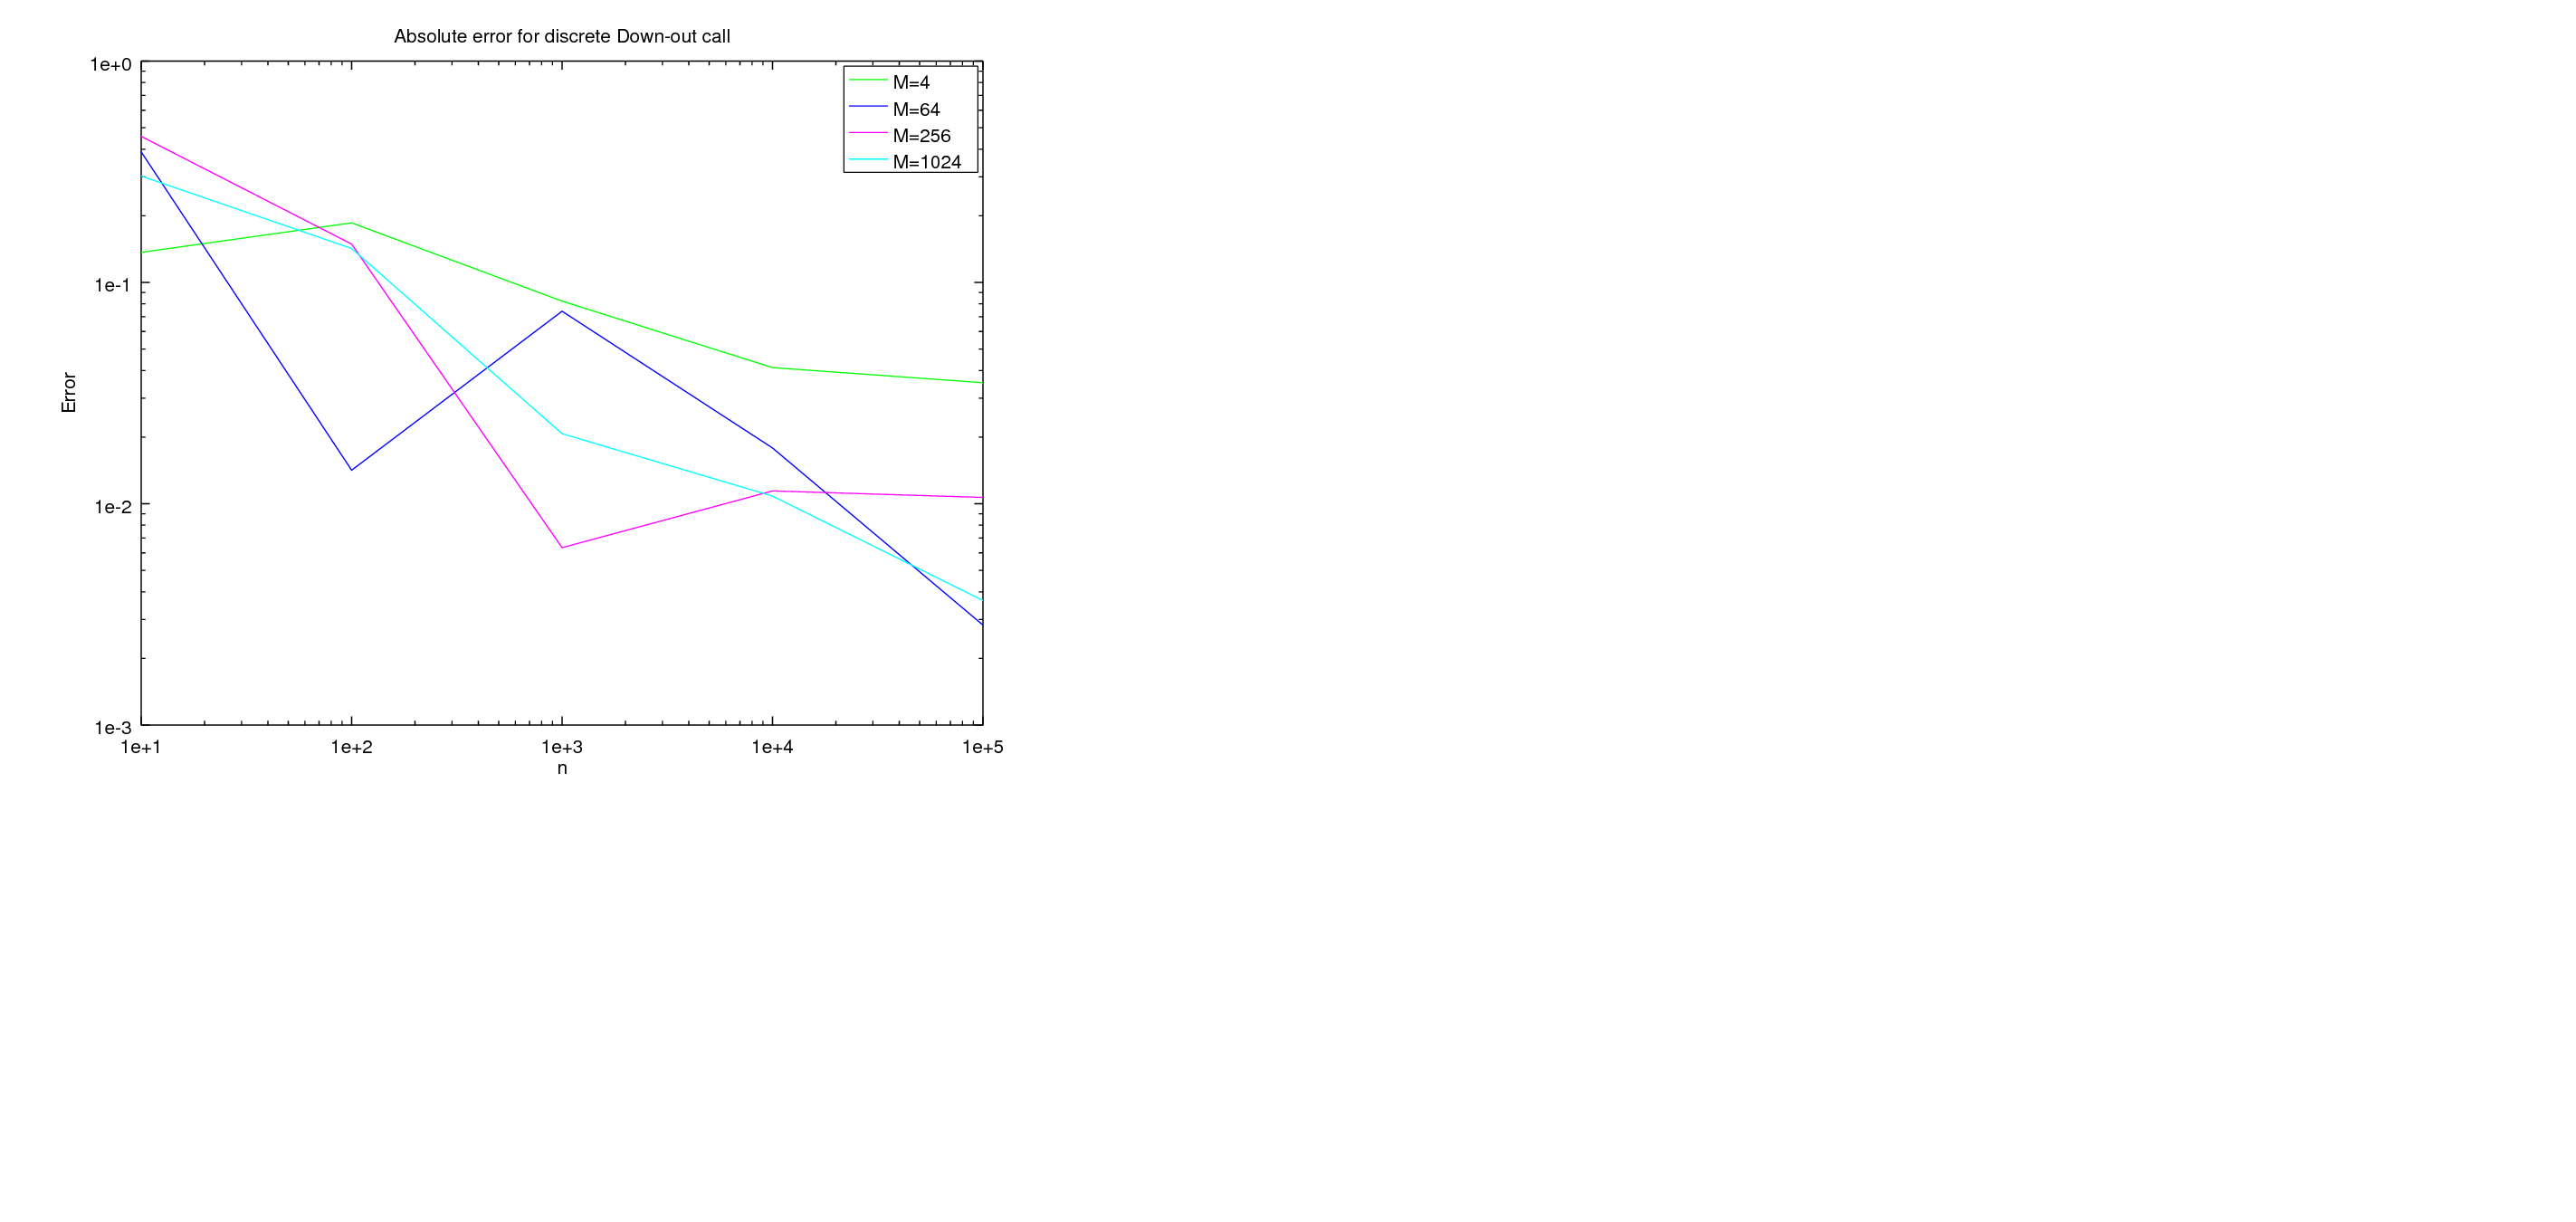
\includegraphics[scale=0.5]{convergence_plot_discrete_down_out_call.png}
\end{center}

\section*{Task 5}

\begin{center}
	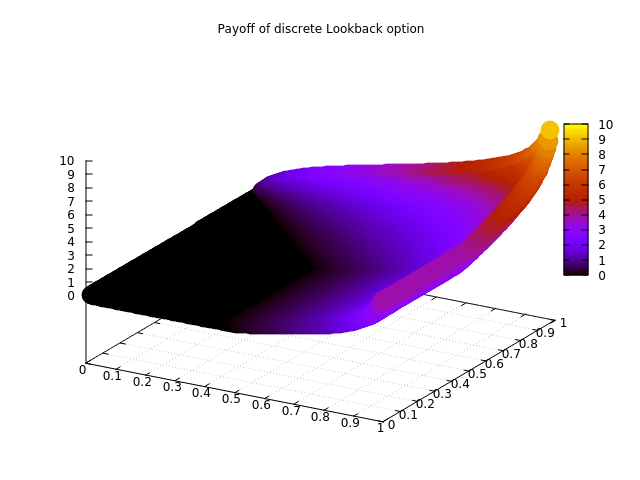
\includegraphics[scale=0.4]{payoff_lookback.png}
\end{center}

\section*{Task 6}

\begin{center}
	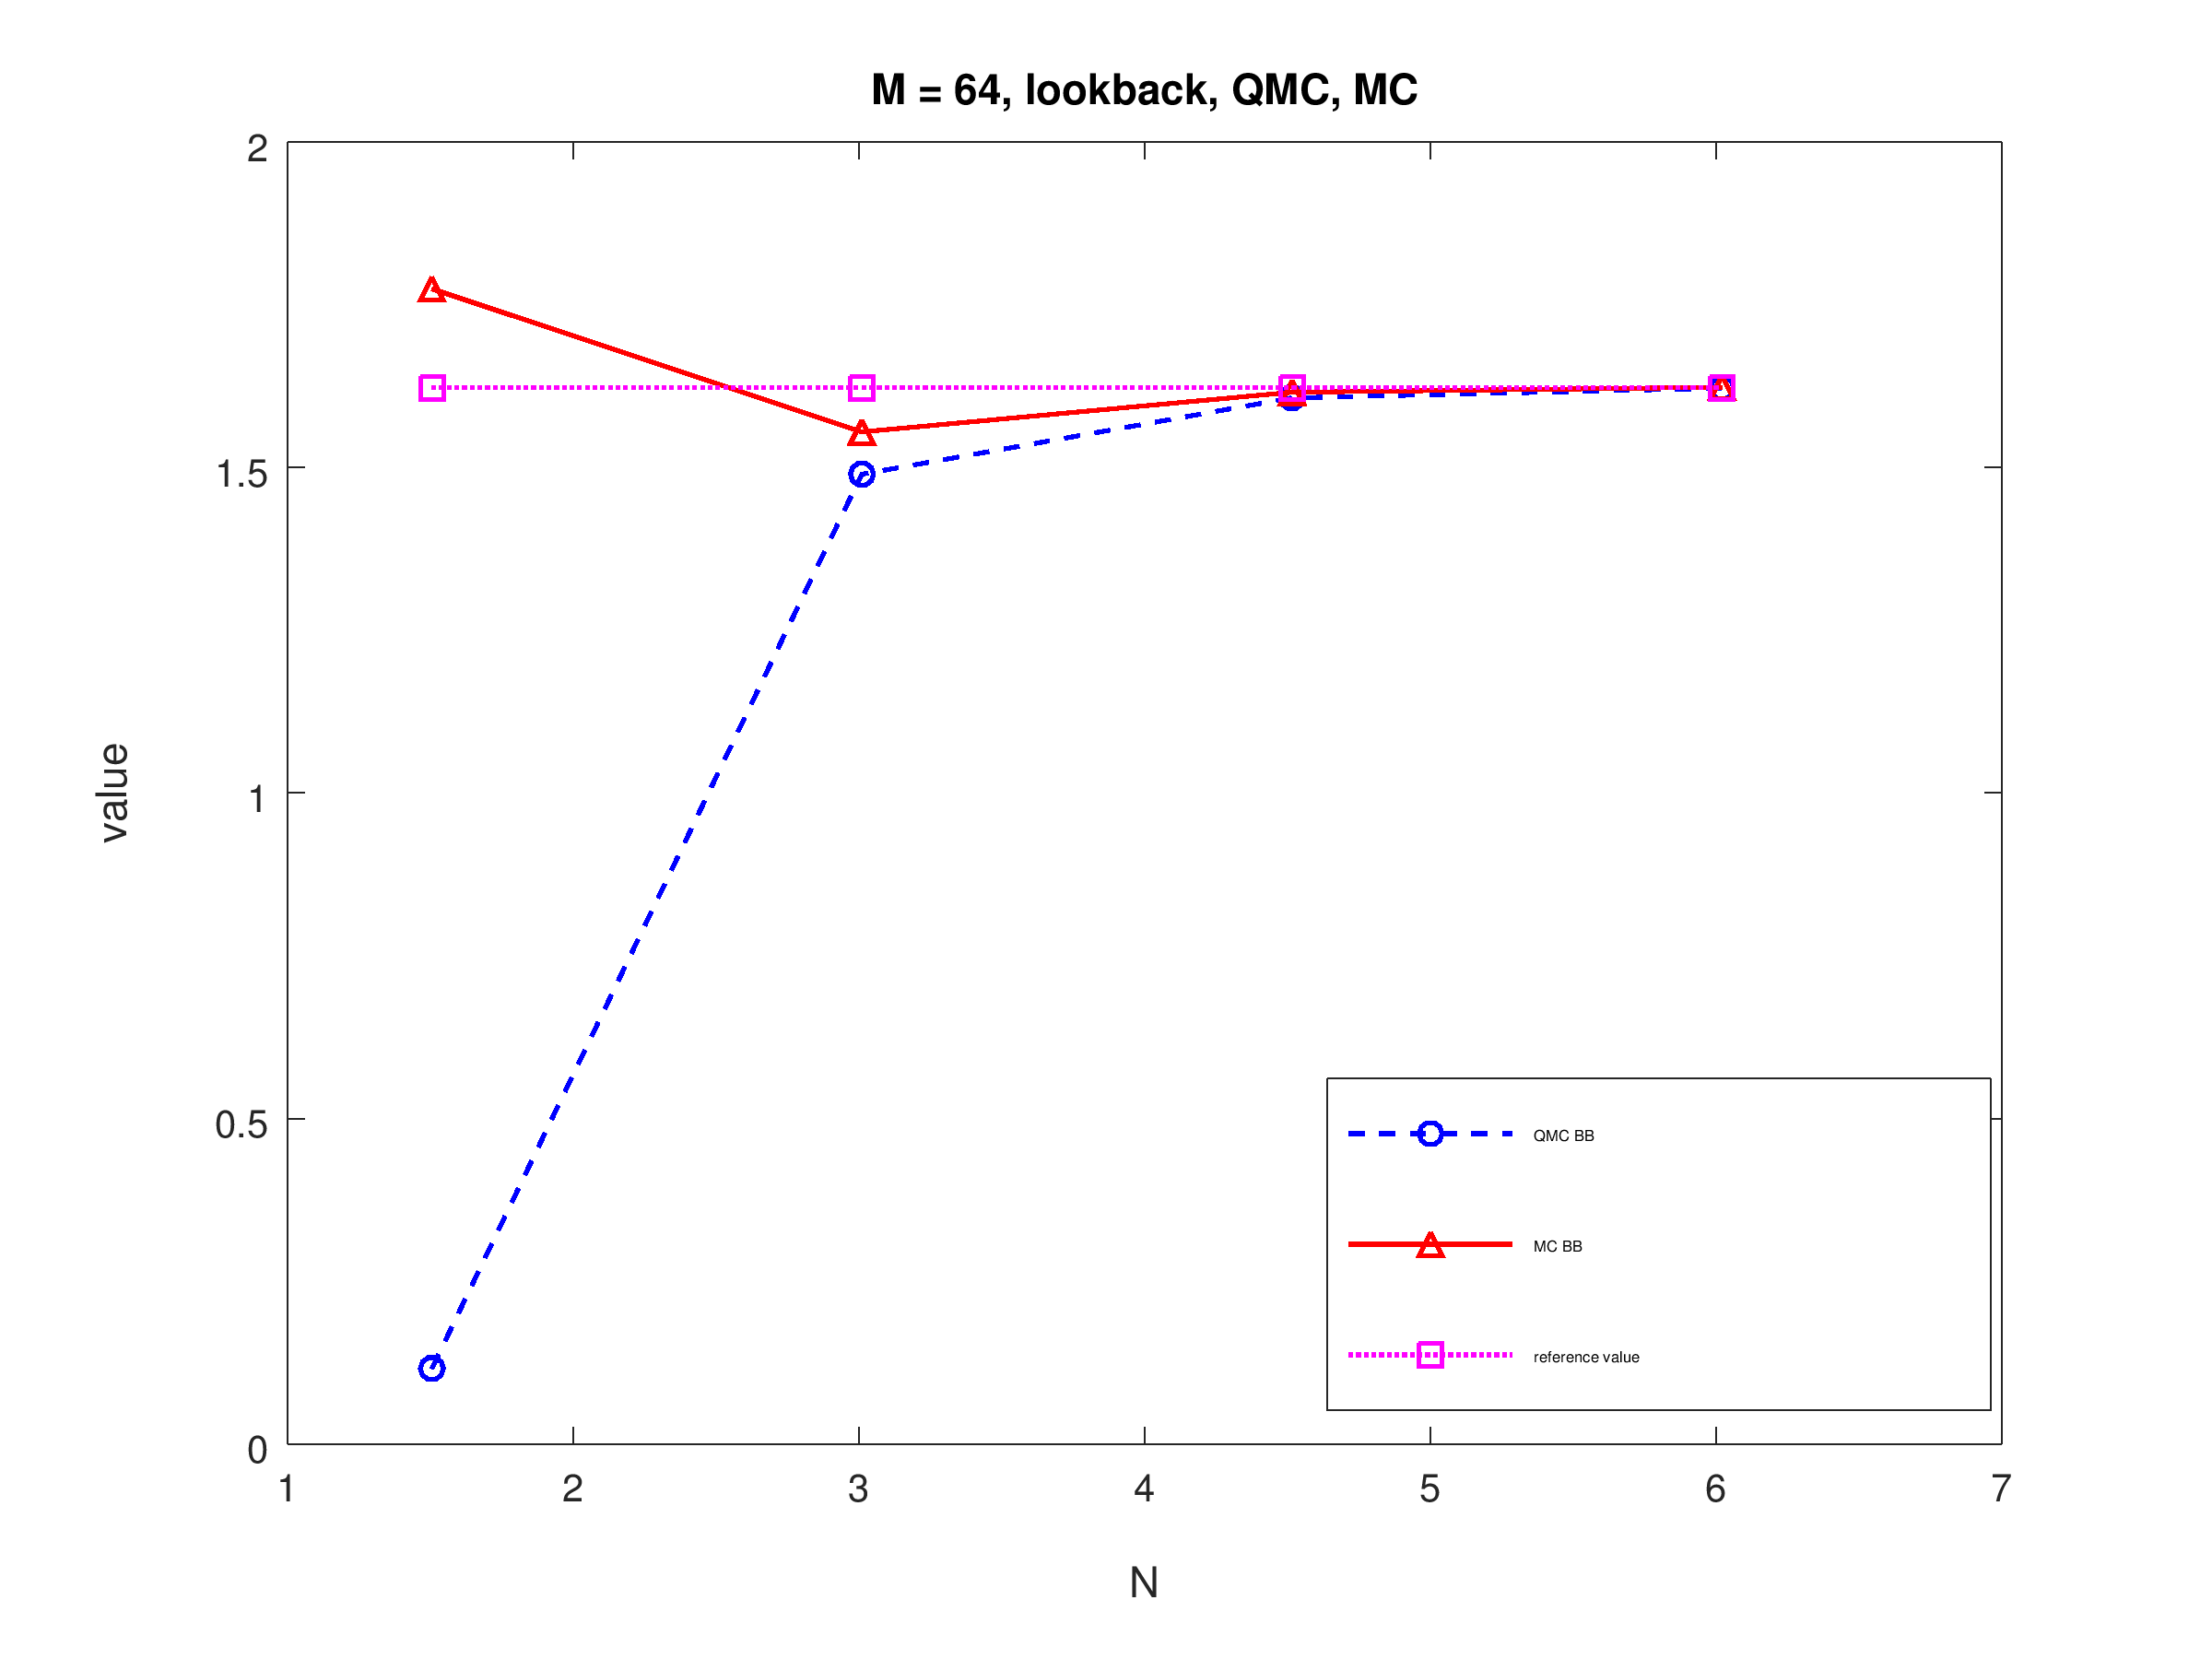
\includegraphics[scale=0.35]{images/task6.png}
\end{center}
\begin{itemize}
    \item{
        On this figure the value of Lookback Call Option computed with QMC and MC methods using Brownian-Bridge is plotted against the number of points used
        
    }
     
\end{itemize}
Here, once more, error between the reference value computed numerically and the value computed with QMC and MC using Brownian-Bridge against number of points.
\begin{center}
	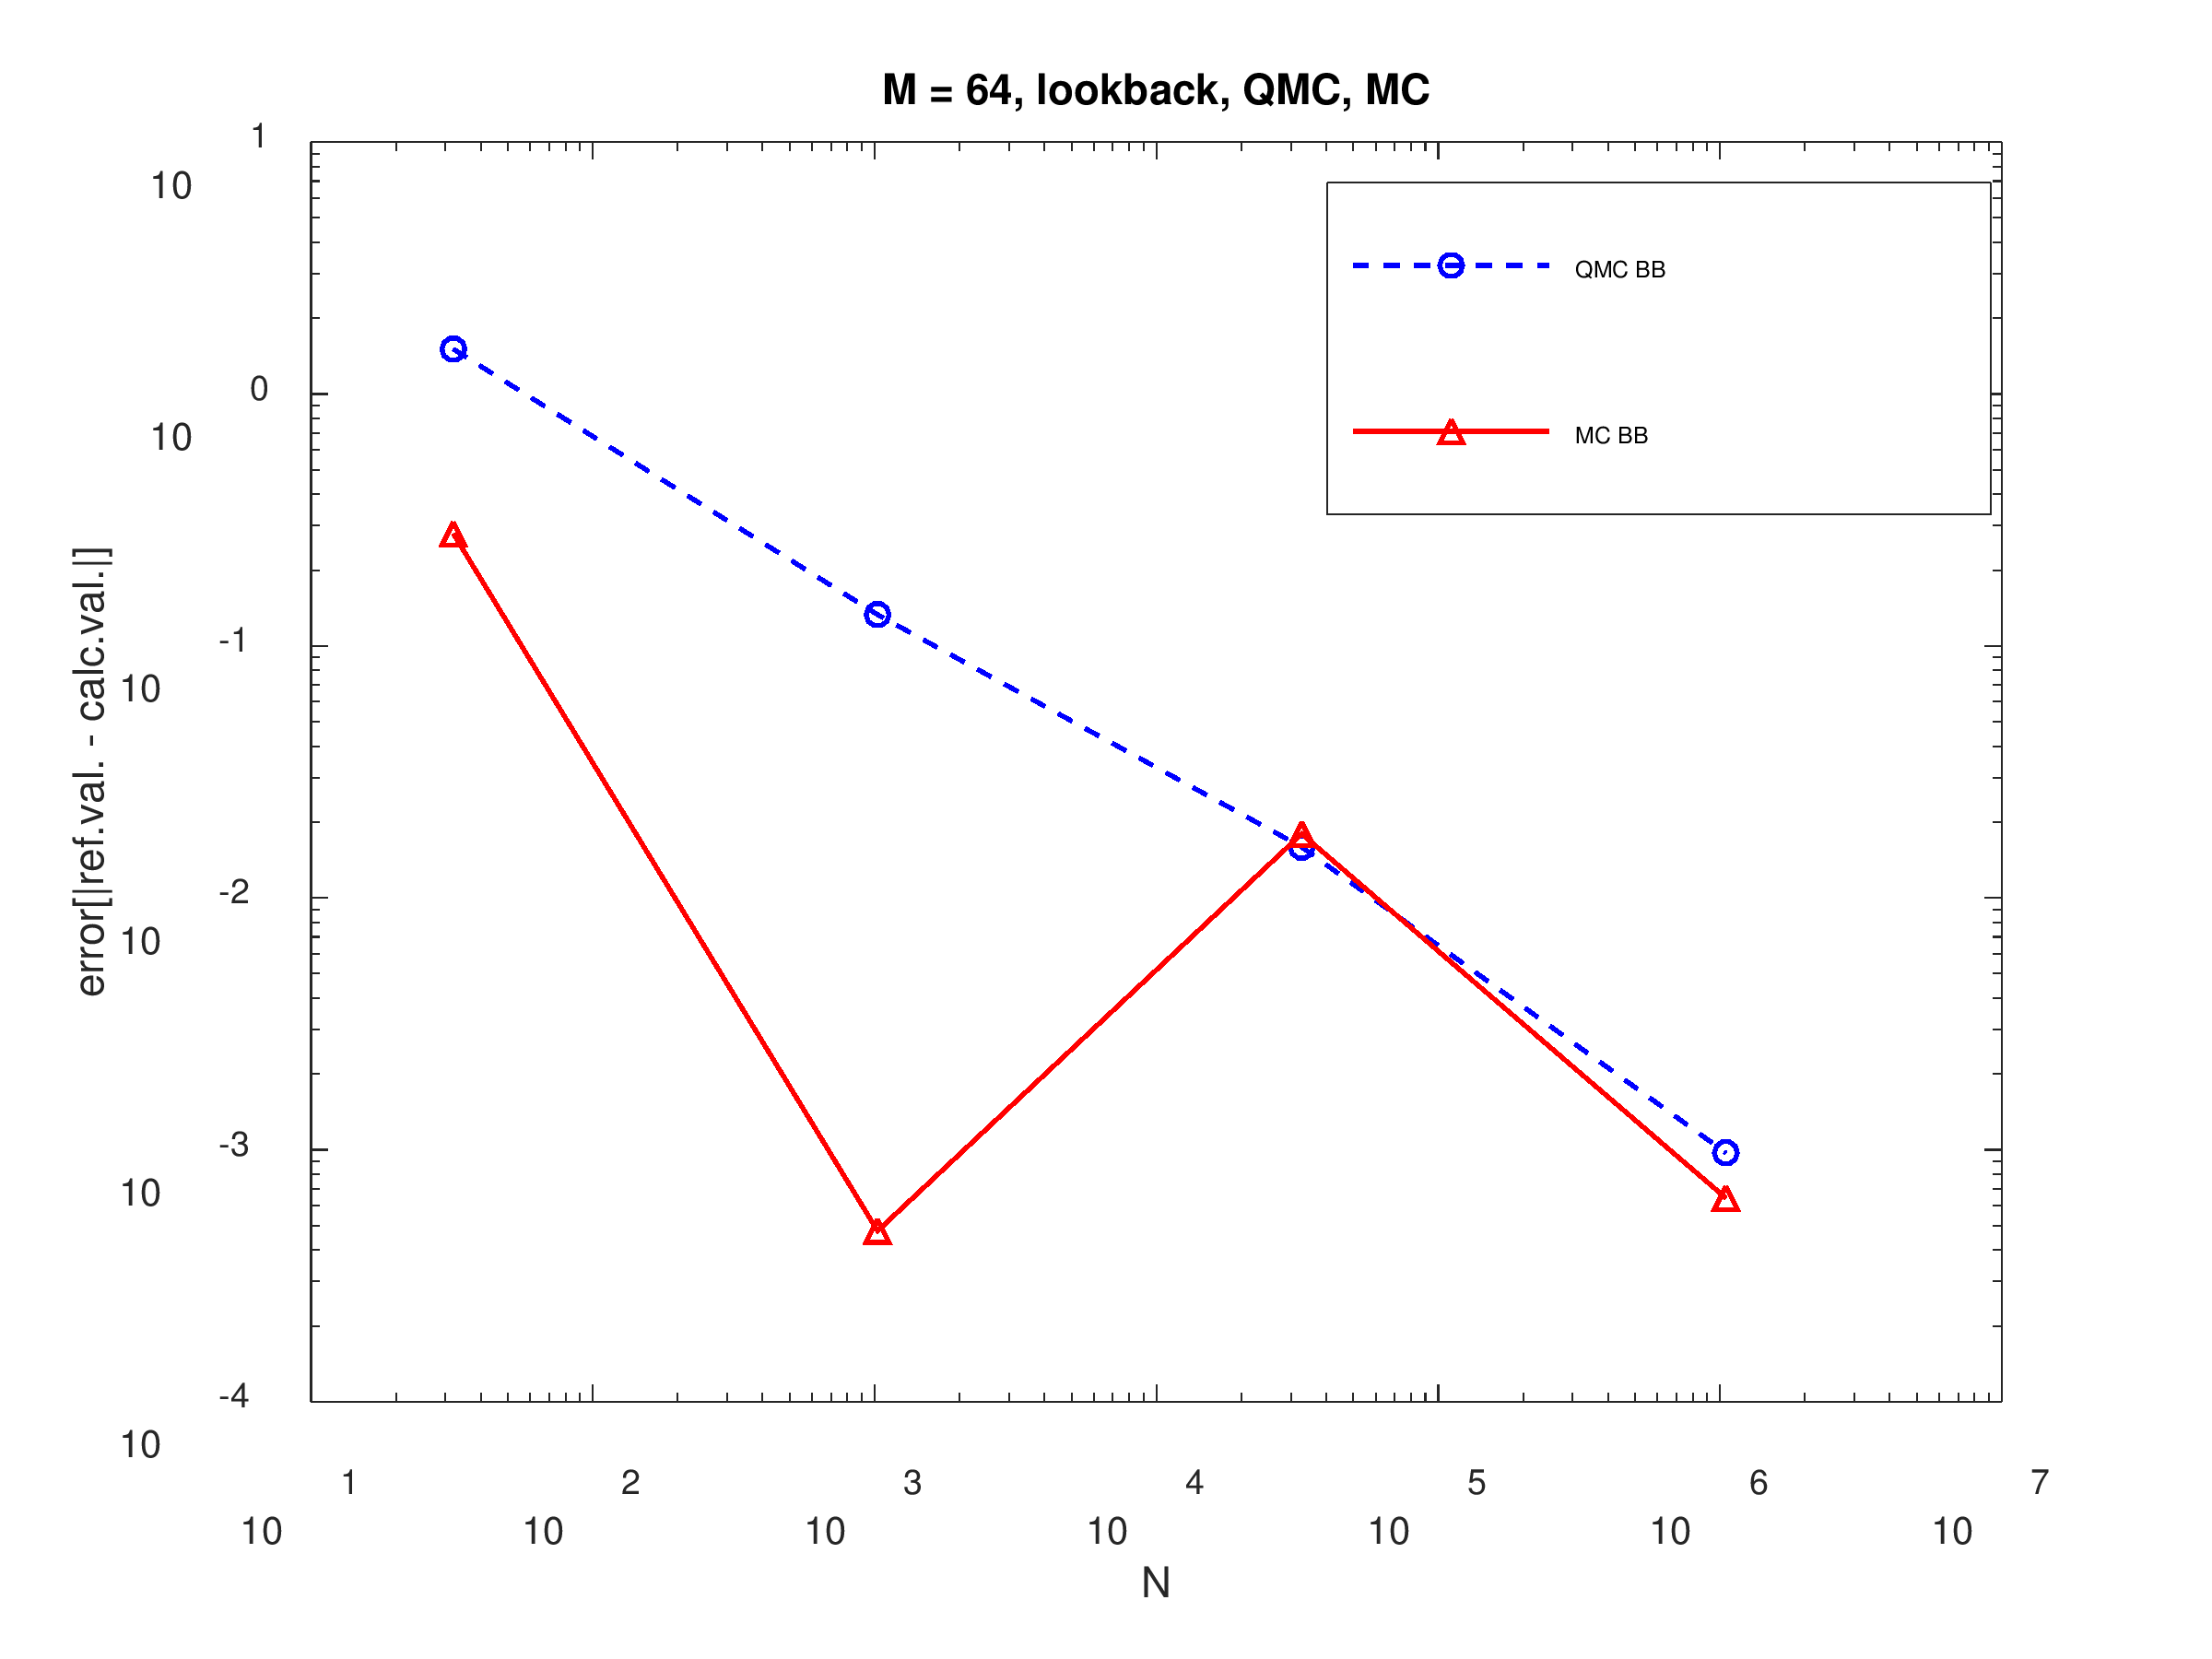
\includegraphics[scale=0.25]{images/task6_error.png}
\end{center}

\section*{Task 7}


\begin{center}
	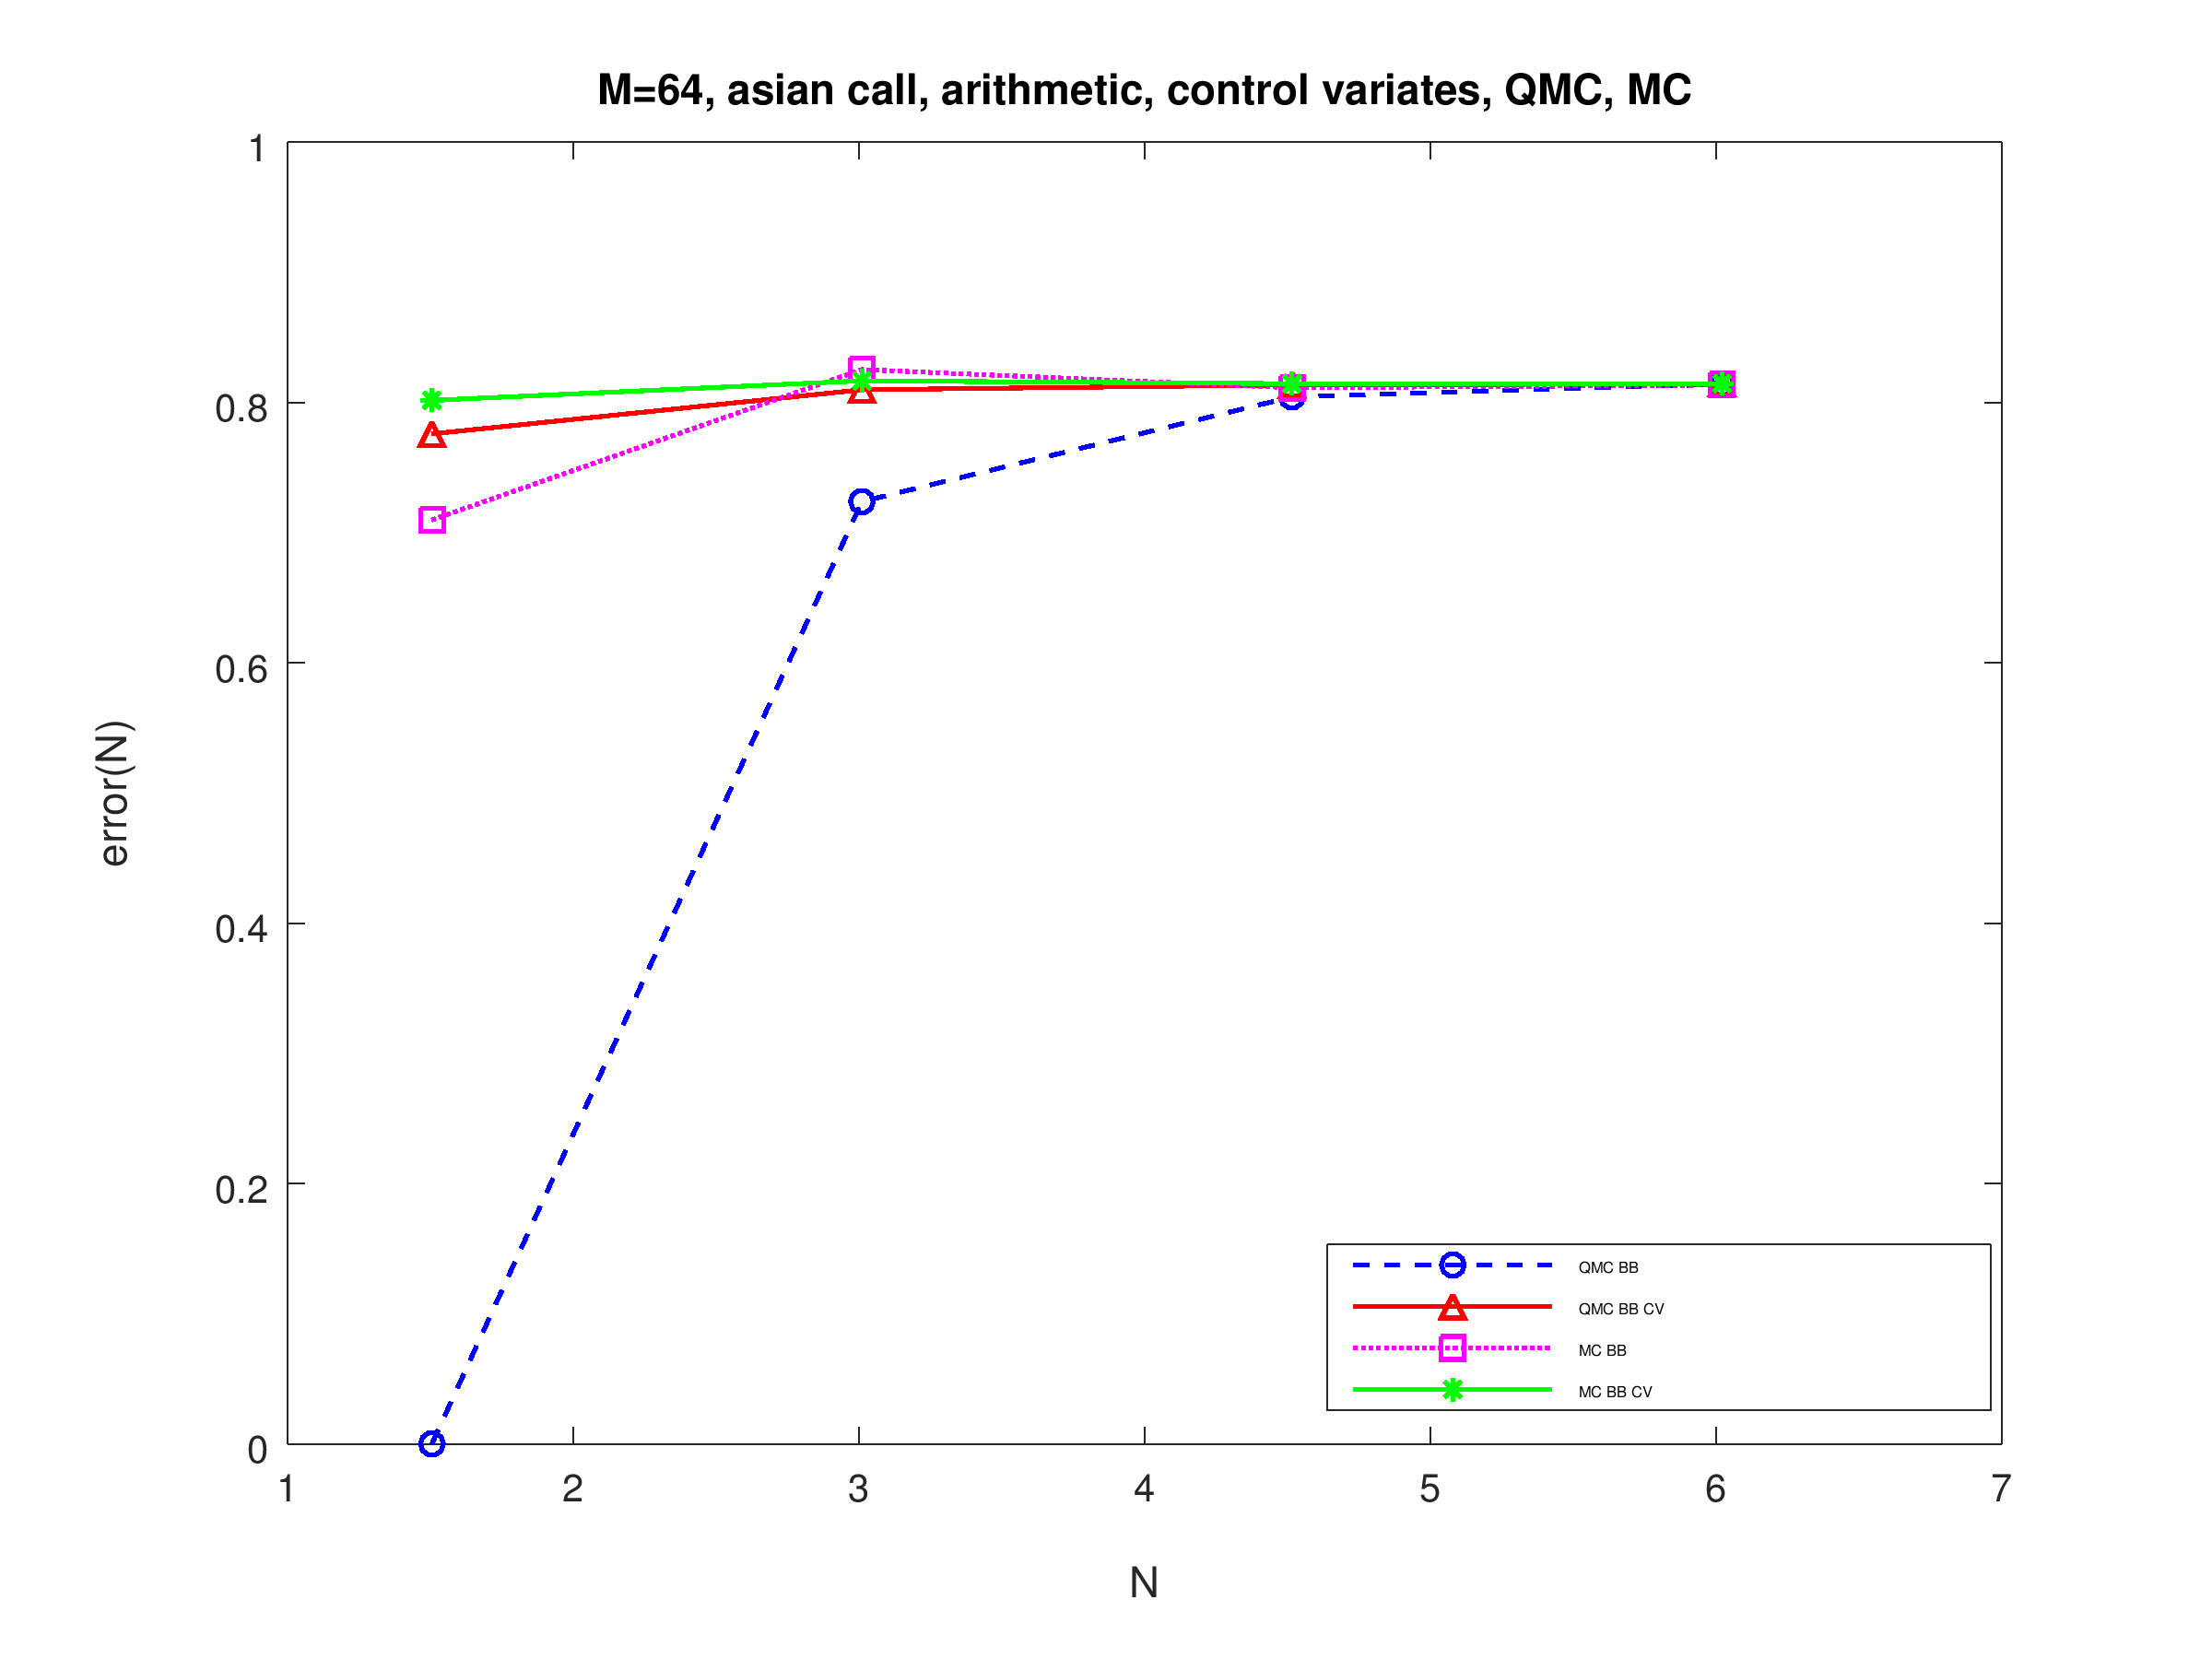
\includegraphics[scale=0.25]{images/task7.png}
\end{center}
\begin{itemize}
    \item{
        On this figure, results of the \textbf{control variate}
        method are presented. The idea was presented on the worksheet, we observe that this method improves variance slightly in case of an arithmetic Asian Call Option. 
    }
\end{itemize}

\section*{Task 9}

\begin{center}
	\includegraphics[scale=0.45]{images/DAX.pdf}
\end{center}

Volatility of Call-Options for DAX, expiring in December, 2017. In this case, the volatility smile is clearly visible. The current value of the DAX is at about $12450$ points. 

\end{document}

